% 2008 年陕西卷理科第 9 题：α⊥β，α∩β=l，A∈α、B∈β，A、B 到 l 的距离为 a、b，
%   AB 与 α、β 所成角为 θ、φ，射影长 m、n，且 a>b。
% 来源 PDF：gaokaomath-src/普通高考/2008/2008陕西理.pdf
% SHA-256：b6b5dd7225debdf38e60611a7b85eebe815344d38958aab6fa987ccea836dec9
% 原页：2008陕西理.pdf 第 1 页（A3 三栏）第 1 栏，书页码 475。
% 绘制依据：按原页的「α 竖起、β 平置、l 为二者交线」关系作图；原页两垂足画在同一处属示意，
%   本图把 A、B 到 l 的两条垂线段分别画出（这是 a、b 的定义，且 α⊥β 时二者一般不在同一点），
%   标注 a、b 分别贴在这两条垂线段旁，AB 为连线。
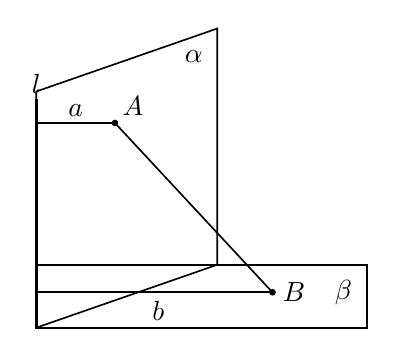
\begin{tikzpicture}[scale=1.0, semithick, every node/.style={inner sep=1.5pt}]
  % α（竖直半平面）
  \draw (0,0) -- (0,3.0) -- (2.3,3.8) -- (2.3,0.8) -- cycle;
  \node at (2.0,3.45) {$\alpha$};
  % β（水平半平面）
  \draw (0,0) -- (0,0.8) -- (4.2,0.8) -- (4.2,0) -- cycle;
  \node at (3.9,0.45) {$\beta$};
  % 交线 l
  \draw[line width=1.0pt] (0,0) -- (0,2.9) node[above] {$l$};

  \coordinate (A) at (1.0,2.6);
  \coordinate (Ap) at (0,2.6);
  \coordinate (B) at (3.0,0.45);
  \coordinate (Bp) at (0,0.45);

  \draw (A) -- (Ap);
  \draw (B) -- (Bp);
  \draw (A) -- (B);

  \fill (A) circle (1.2pt); \node[above right=1pt] at (A) {$A$};
  \fill (B) circle (1.2pt); \node[right=2pt] at (B) {$B$};
  \node[above] at (0.5,2.62) {$a$};
  \node[below] at (1.55,0.40) {$b$};
\end{tikzpicture}
